\documentclass{article}

\usepackage{indentfirst}
\usepackage{amsmath}
\usepackage{graphicx}
\usepackage{hyperref}
\usepackage[utf8]{inputenc}
\usepackage{lipsum}
\usepackage[a4paper]{geometry}
\usepackage{xcolor}
\usepackage{listings}
\usepackage{natbib}
\lstset{
    basicstyle=\ttfamily,
    showstringspaces=false,
    commentstyle=\color{red},
    keywordstyle=\color{blue}
}
\graphicspath{{}}
\geometry{
    left=20mm,
    top=20mm,
}
\renewcommand{\thesection}{\Roman{section}}
\renewcommand{\thesubsection}{\Roman{subsection}}
\title{\LARGE \textbf {\huge{Mendalami Onion Network dengan TOR}}}
\author{
    M Rizqi R\\
    20051204034\\
    Teknik Informatika 2020 B\\
    Universitas Negeri Surabaya\\
    \and
        Alfito Mulyono\\
        20051204038\\
        Teknik Informatika 2020 B\\
        Universitas Negeri Surabaya\\
}
\date{\today}
\usepackage{hyperref}
\begin{document}
    \maketitle
        \section{Pendahuluan}
        \subsection*{1.1 Latar Belakang}
        Bocornya informasi pengguna internet memiliki dampak yang merugikan.
        Banyak sekali pihak yang ingin mencuri data kita untuk 
        dimanfaatkan dalam kepentingan mereka pribadi. Mereka akan menjual 
        data kita kepada pihak-pihak yang menginginkan data kita.

        Kita dapat mengambil contoh dari sebuah perusahaan media sosial ternama
        seperti Facebook. Pada 19 Desember 2018, Facebook diketahui telah
        membocorkan 1,5 miliar data pengguna Facebook dan menjualnya kepada pihak ketiga.
        Mark Zuckerberd, pendiri Facebook dinyatakan bersalah dalam persidangan 
        dan dijatuhi denda sesuai keputusan hakim.

        Namun kebocoran data bisa juga terjadi karena kesalahan pengguna.
        Pengguna kerap mengunjungi situs-situs acak kemudian tanpa
        sengaja menekan iklan yang muncul dalam situs tersebut. 
        Kemudian pengguna tanpa sadar telah mengunduh perangkat
        lunak yang berisi virus yang kemudian berjalan dibelakang layar.
        Virus ini dapat berupa berbagai jenis perangkat lunak yang dapat
        menginfeksi perangkat pengguna.

        Ada pula virus yang bahkan bisa digunakan untuk melacak setiap jengkal
        aktivitas pengguna. Baik itu dari ketikan keyboard, lokasi, bahkan mampu memanipulasi
        berkas digital yang dimiliki oleh pengguna hingga bisa mencuri berkas tersebut.

        Maka dari itu diperlukan cara agar kita terhindar dari kejahatan internet tersebut.
        Salah satunya ialah memilih alat penjelajah web (\textit{web browser}) yang tepat.
        Web browser yang tidak melacak kita saat menjelajah internet dan mencegah
        situs-situs berbahaya melacak dan mencuri data kita.
        \subsection*{1.2 Rumusan Masalah}
        \noindent Adapun rumusan masalah pada pemaparan ini adalah:
        \begin{enumerate}
            \item Apa yang dimaksud dengan keamanan internet?
            \item Bagaimana mencegah diri dari \textit{cyber crime}?
            \item Bagaimana menggunakan TOR sebagai media penjelajah yang aman?
        \end{enumerate}

        \subsection*{1.3 Tujuan}
        \noindent Berdasarkan latar belakang yang telah dipaparkan. Tujuan makalah ini adalah
        untuk memberikan wawasan tentang \textit{web browser} yang fokus pada 
        privasi dan keamanan pengguna. Maka dari itu, tujuan spesifik dari makalah
        berikut adalah sebagai berikut:
        \begin{enumerate}
            \item Membuat pembaca mengerti tentang pentingnya \textit{cyber security.}
            \item Membuat pembaca memahami cara mengamankan dirinya dari kebocoran dan pencurian data.
            \item Membuat pembaca memahami konsep \textit{Cyber Security, VPN, proxy, TOR Network}.
            \item Membuat pembaca memahami cara menggunakan \textit{TOR Network}. 
        \end{enumerate}
       
        \section{Pembahasan}
        \subsection*{2.1 Cyber Security}
        \noindent Adalah istilah yang digunakan untuk metode pengamanan data baik pribadi
        maupun publik dalam jaringan internet. Metode \textit{cyber security}
        dirancang untuk melawan ancaman terhadap sistem jaringan dan aplikasi,
        baik itu serangan yang berasal dari dalam maupun luar sistem.
        \subsection*{2.2 VPN}
        Adalah singkatan dari \textit{Virtual Private Network} merupakan
        sebuah metode untuk menyembunyikan alamat IP asli dari pelacakan. Dengan VPN
        , alamat IP akan dipalsukan atau dialihkan dari perangkat asli pengguna
        ke perangkat yang ada di server penyedia VPN. Contoh kasusnya
        adalah jika penyedia internet kita mencegah kita untuk mengakses
        alamat IP tertentu, maka kita bisa memakai VPN untuk melakukan 
        tunneling ke sever luar yang dimana alamat IP tersebut bisa di akses.
        Dengan ini, alamat IP pengguna yang sesungguhnya dapat di bungkus
        dan dialihkan ke alamat IP server luar atau pihak ketiga.
        Namun metode ini tidak sepenuhnya aman. Sudah banyak laporan tentang
        bocornya data pengguna NordVPN. NordVPN ialah salah satu 
        penyedia layanan VPN yang sudah cukup terkenal. Namun sudah banyak
        laporan bahwa data pengguna bocor.

        Ini disebabkan adanya tindakan penetrasi pada enkripsi saat pengguna
        melakukan autentifikasi ketika mencoba terhubung ke layanan penyedia VPN.
        Kemungkinan yang lain adalah ada yang mengakses server VPN secara langsung
        dan mencuri data atau kunci autentifikasi pengguna. Juga bisa terjadi ketika
        pengguna mengakses Wi-Fi publik yang ternyata merupakan Wi-Fi buatan peretas 
        dan peretas tersebut mendapatkan kunci VPN melalui \textit{Man In The Middle Attack}.
        \subsection*{2.3 Proxy}
        \noindent Adalah sebuah server pihak ketiga yang menjadi perantara antara
        pengguna ke server yang dituju sebagai alternatif daripada 
        langsung menghubungi server. Proxy ditujukan bila pihak penyedia
        internet memblokir alamat IP tertentu. Maka dengan proxy, kita bisa
        terlebih dahulu terhubung ke server pihak ketiga kemudian mengakses 
        alamat IP tujuan kita melalui server tersebut. Namun metode ini 
        tidak akan menyembunyikan alamat IP kita dan cenderung rawan untuk 
        dipenetrasi dengan \textit{Man In The Middle Attack.} Seseorang bisa sengaja
        masuk diantara jalur pengguna dan penyedia \textit{proxy} dan 
        melakukan \textit{sniffing} atau melihat data yang lewat melalui 
        jaringan.

        \subsection*{2.4 TOR Network}
        TOR (The Onion Routing) adalah sebuah \textit{Free and Open Source Software} yang merupakan sebuah 
        protokol keamanan diinternet yang bisa digunakan secara gratis. Protokol ini akan
        menggabungkan teknologi \textit{VPN} dan \textit{Proxy}. Dimana pengguna akan masuk
        ke dalam jaringan TOR untuk mengakses internet. Alamat IP pengguna akan melompati 
        beberapa server sukarelawan secara acak sebelum terhubung ke internet.
        \begin{figure}[h]
        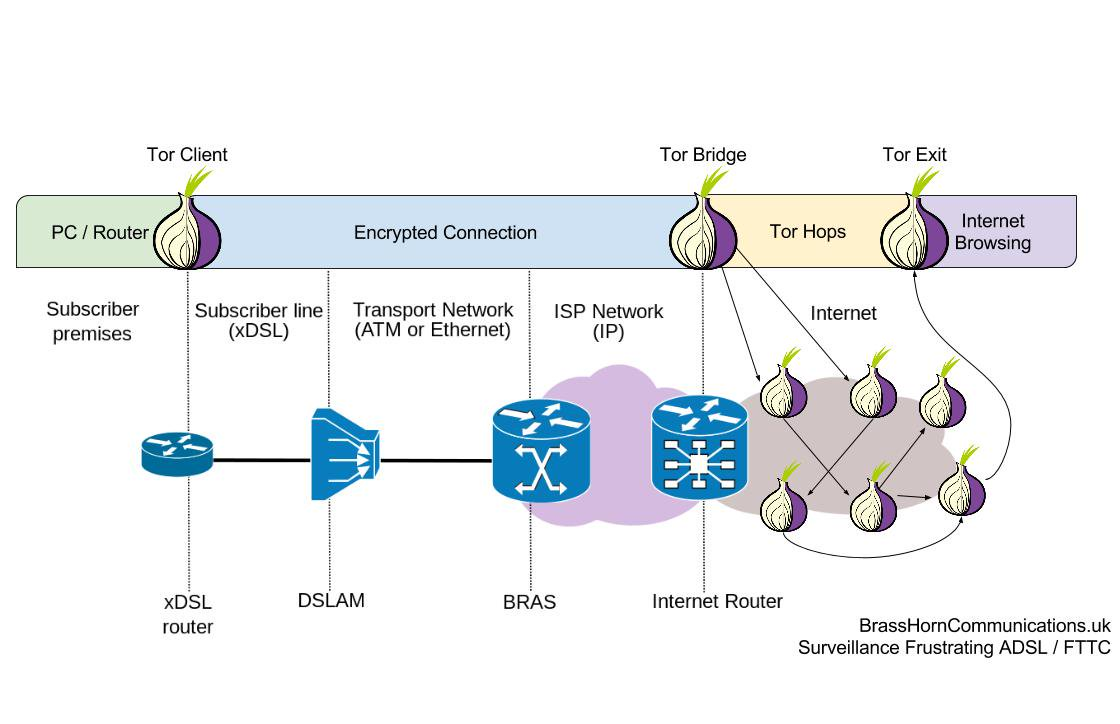
\includegraphics[scale=0.5, width=0.5\textwidth]{tor.jpg}
        \centering 
        \end{figure}

        Ini dapat memberikan keamanan lebih kepada pengguna dikarenakan alamat IP pengguna
        akan dibungkus dengan berlapis-lapis alamat IP yang membuat penyerang kesulitan bahkan
        tidak mungkin melacak alamat IP asli pengguna. Ini juga dikarenakan fitur enkripsi
        akan diterapkan pada setiap pembungkus alamat IP. Semua ini bisa dilakukan dengan 
        menggunakan TOR Browser atau TOR Tunneling.

       \subsection*{2.4.1 Instalasi TOR Browser } 
       Kita dapat menggunakan TOR dengan menginstall TOR Browser yang bisa didapatkan melalui 
        situs resmi yaitu \url{https://www.torproject.org/}.

        \begin{figure}[h]
        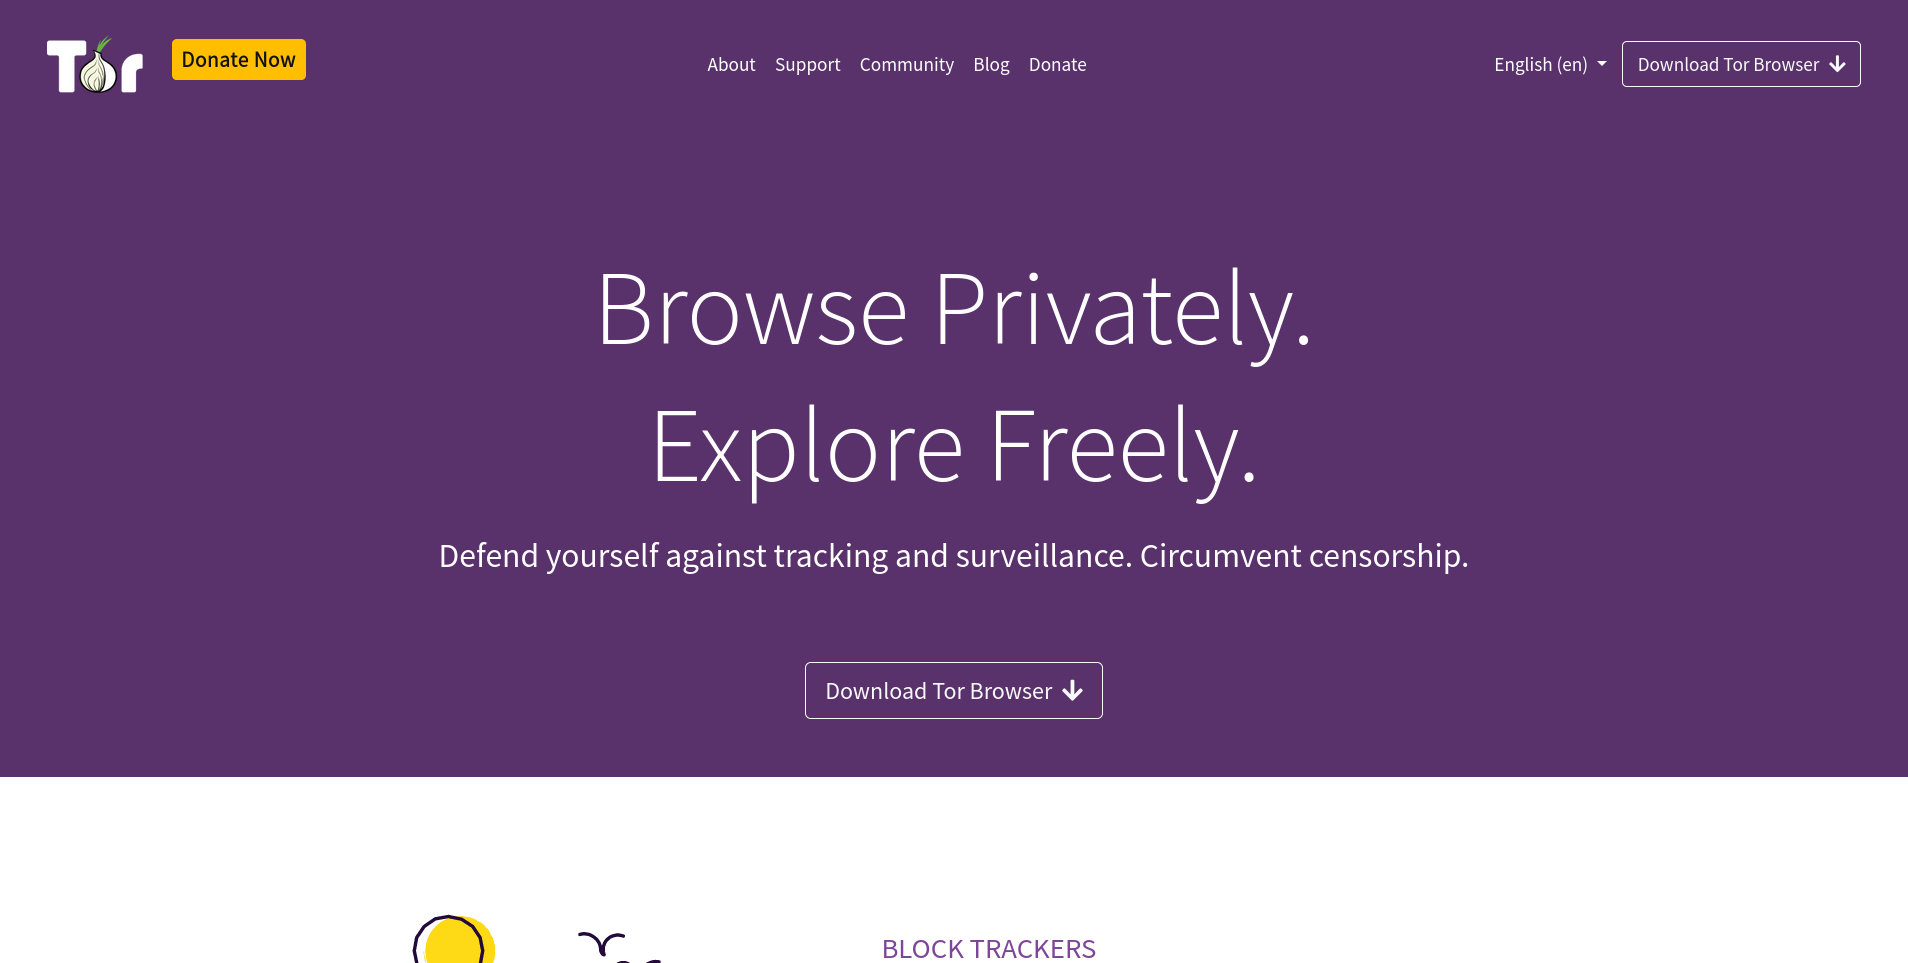
\includegraphics[scale=0.5, width=0.5\textwidth]{tor-web.png}
        \centering 
        \end{figure}

        Kemudian masuk ke laman \textit{Download} dan pilih sistem operasi yang digunakan.
        Setelah selesai mendownload, jika pengguna menggunakan Sistem Operasi Windows, maka
        TOR Browser dapat diinstal dengan melalui file yang telah di download. 
        Untuk Sistem Operasi Distribusi Linux, TOR Browser tersedia di \textit{Package Manager}
        setiap distro atau dapat diinstall melalui Flatpack atau Snap Packages.

        Jika tidak tersedia, maka kita bisa langsung masuk ke situs resmi dan mendownload
        \textit{executable binnary}.

        \begin{figure}[h]
        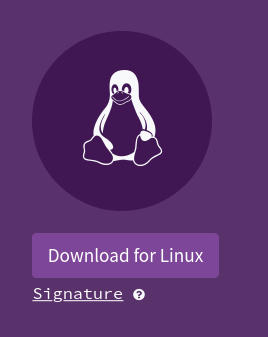
\includegraphics[scale=0.3]{tor-linux.png}
        \centering
        \end{figure}

        Setelah terdownload, navigasi ke folder tempat file kompresi tersebut berada dan
        extract menggunakan perintah :
        \begin{lstlisting}[language=bash]
           tar -xvf tor-browser-linux64-11.0.6_en-US.tar.xz 
        \end{lstlisting}
        Sesuaikan versi dengan yang telah didownload. Kemudian masuk ke directory tersebut
        dan eksekusi dengan :
        \begin{lstlisting}[language=bash]
            ./start-tor-browser.desktop
        \end{lstlisting}
        kemudian akan muncul tampilan seperti berikut :
        \begin{figure}[h]
        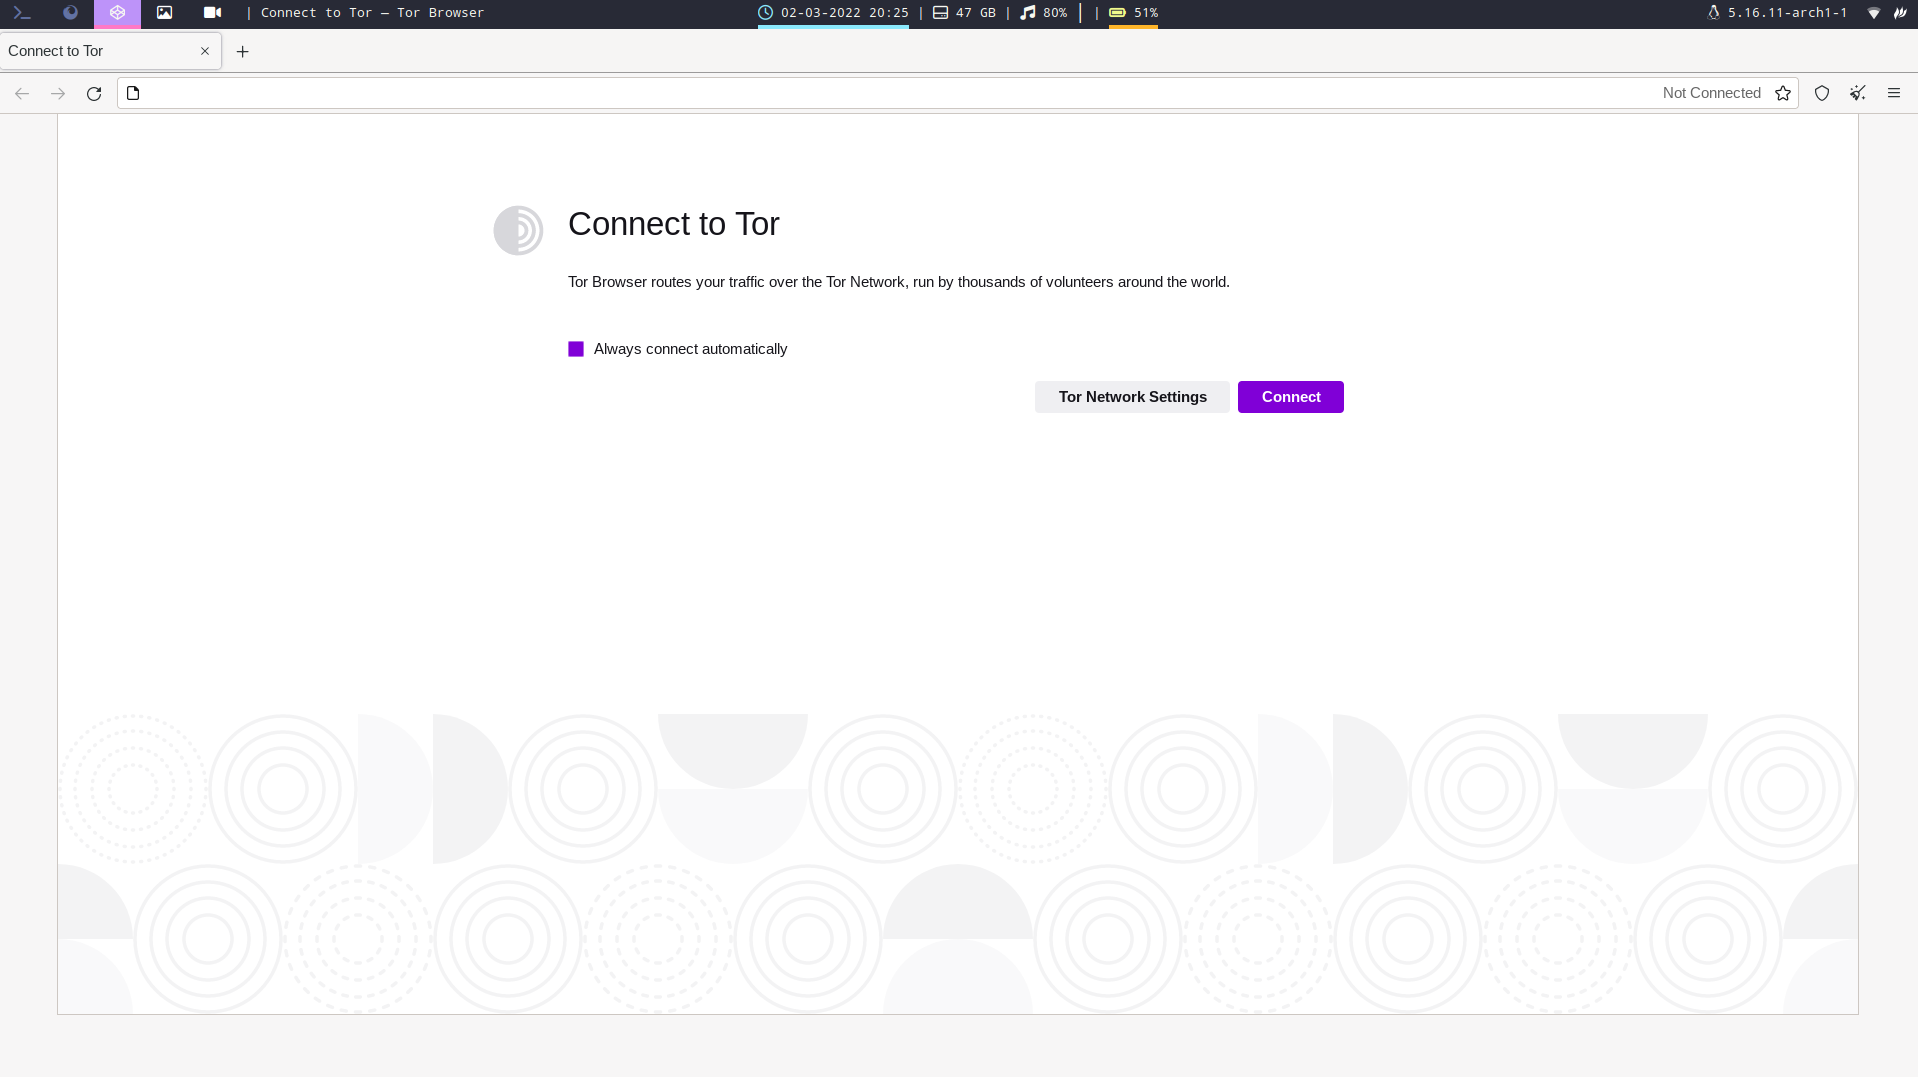
\includegraphics[width=0.5\textwidth]{tor-first.png}
        \centering
        \end{figure}

        Kita bisa langsung memilih 'Connect' untuk menyambungkan ke jaringan TOR.
        Akan membutuhkan sedikit waktu untuk terhubung, terutama bila jaringan
        internet pengguna terbilang lambat. Maka waktu yang diperlukan untuk 
        menghubungi TOR Network juga akan lebih lambat. Dikarenakan alamat IP harus
        melompat ke banyak node agar bisa mencapai onion routing.
        Bila sudah terhubung, akan muncul tampilan sebagai berikut :
        \begin{figure}[h]
        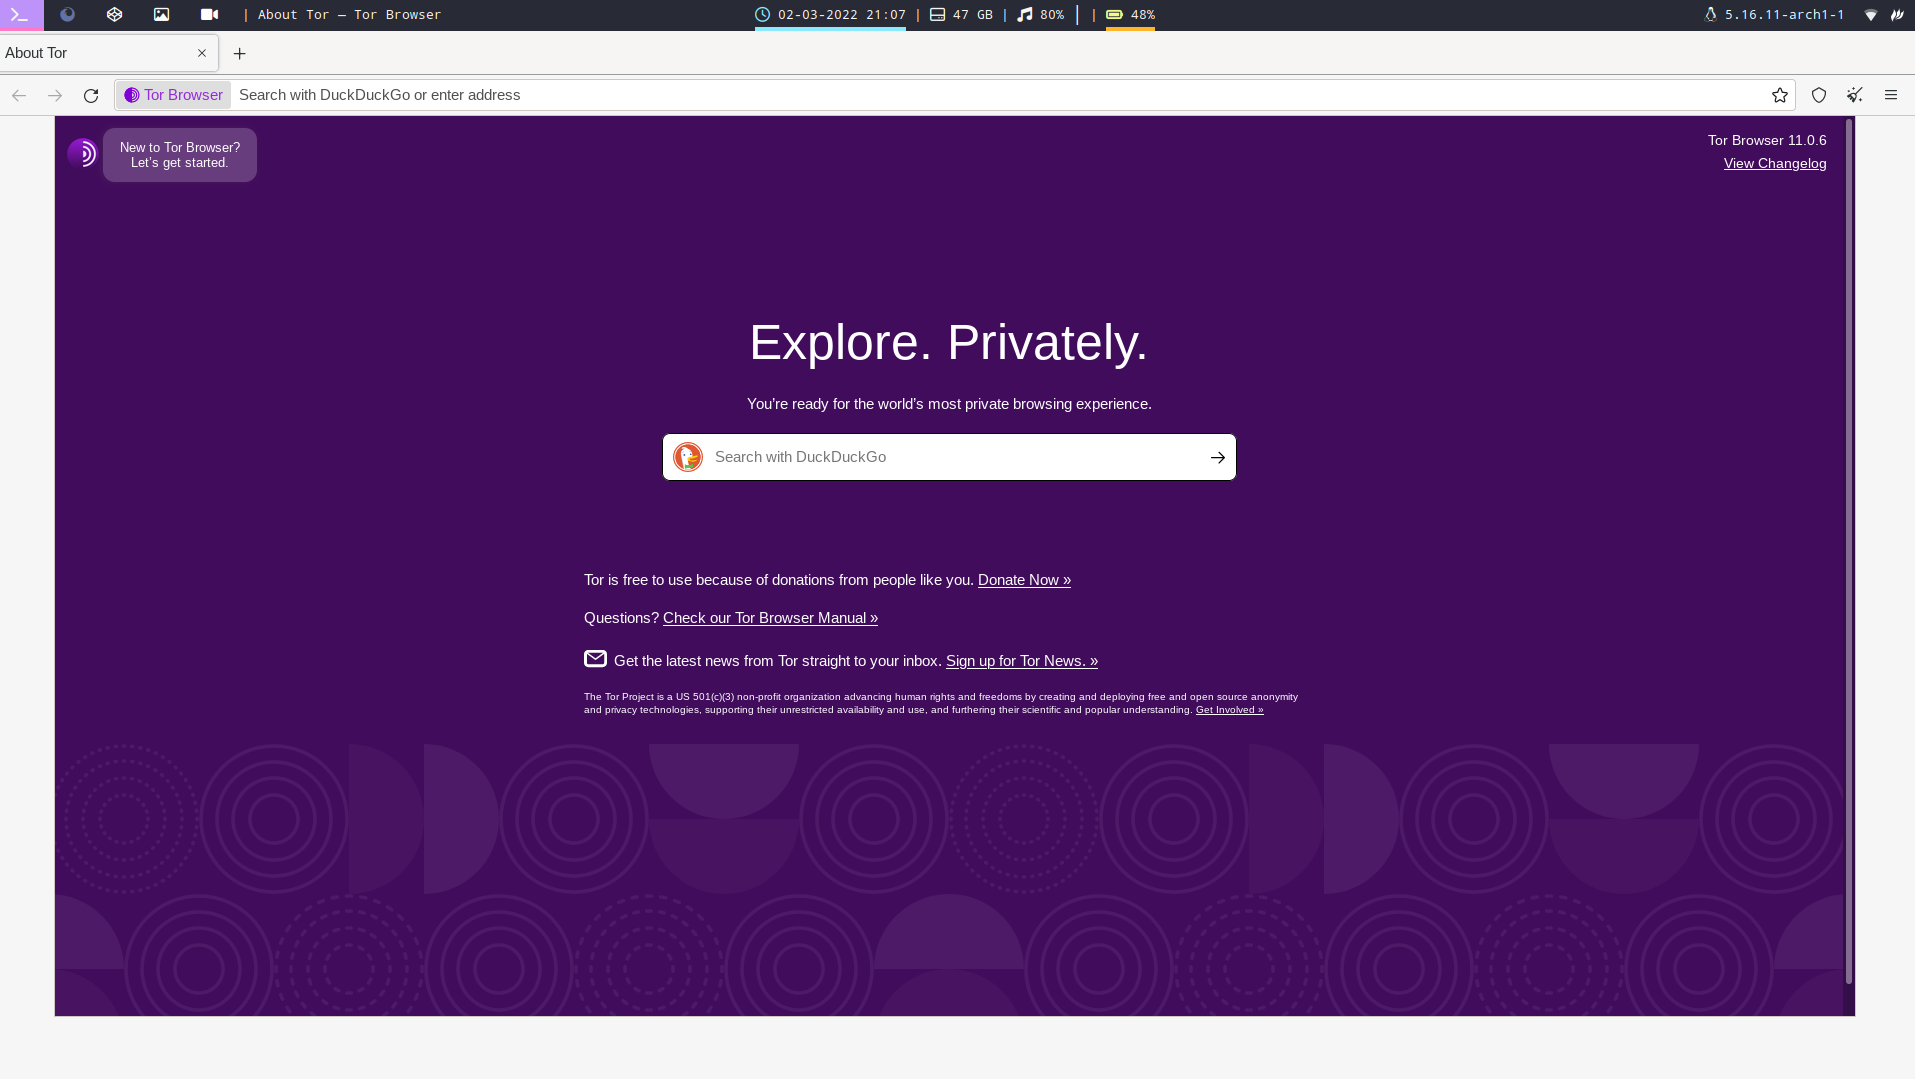
\includegraphics[width=0.5\textwidth]{tor-connect.png}
        \centering
        \end{figure}

        Setelah ini, kita dapat mengakses internet tanpa perlu khawatir dengan adanya
        pelacakan. Dengan TOR juga kita dapat mengakses situs-situs yang tidak
        biasa ada di internet dengan domain \textit{.onion}. Biasanya situs yang
        menggunakan domain \textit{.onion} merupakan situs-situs tersembunyi berisi 
        layanan ilegal seperti cuci uang, senjata ilegal, penyewaan hacker, pembunuh
        bayaran, dan lain-lain.

        


        \section{Penutup}
        Dengan ini dapat dikatakan bahwa untuk mencegah diri dari \textit{cyber attack}.
        terdapat berbagai metode. Beberapa diantaranya ialah menggunakan \textit{proxy, VPN, dan TOR}.
        untuk menyembunyikan identitas kita di internet dan mencegah penjahat untuk
        melacak aktivitas dan keberadaan kita. Namun cara diatas tidak akan berhasil jika
        tidak disertai dengan kesadaran berinternet yang memadai dan mawas akan teknologi.
        Melakukan tindakan seperti mendownload dan/atau menginstall konten bajakan seperti
        film, perangkat lunak, dan sebagainya juga mampu mendatangkan marabahaya dikarenakan
        kita tidak bisa memastikan apakah file tersebut aman dari virus atau perangkat
        lunak berbahaya lainnya.

        Selain itu, juga lebih banyak metode yang biasa digunakan oleh para kriminal
        untuk mengakses data kita. Namun karena hal tersebut barada diluar konteks
        pembahasan tulisan ini, maka penulis tidak mencantumkan penjelasan lebih lanjut
        mengenai metode yang digunakan. Selama kita berhati-hati dalam menjelajah internet
        maka kita akan mendapatkan keamanan dan kenyamanan yang kita inginkan dan kita butuhkan.

        Sekian yang dapat penulis sampaikan. Kurang dan lebihnya mohon dimaafkan dikarenakan
        penulis juga hanya manusia biasa yang tak luput dari kesalahan.
        \textbf{Terima kasih.}

        \nocite{*}
        \bibliographystyle{plainnat}
        \bibliography{Biblio}
        
        \end{document}
        \item Membuat pembaca